

\chapter{Architecture Générale et technologies utilisées}

Ce projet a pour but de fournir un programme permettant de concevoir des bases d'apprentissage automatiquement pour l'entraînement de systèmes de reconnaissance d'écriture manuscrite. Il sera notamment exploité par les \href{http://archives.ille-et-vilaine.fr/fr}{archives d'Ille-et-Vilaine} ainsi que la startup \href{http://www.doptim.eu}{Doptim}. Les reconnaisseurs utilisés pouvant être multiples, il faut que ce projet puisse facilement évoluer, qu'une partie du projet puisse être remplacée par un morceau plus adapté au reconnaisseur choisi. Ainsi, tous les modules de notre projet et non seulement l'interface avec le reconnaisseur doivent pouvoir être remplacés par l'implémentation choisie par l'utilisateur. Par exemple, nous avons choisi une base de données intégrée avec \textit{SQLite} mais celle-ci ne peut gérer facilement l'accès concurrentiel, ou gérer efficacement une grande quantité de données. Ainsi, l'utilisateur pourrait choisir d'utiliser une autre base de données comme \textit{MySQL} ou \textit{MongoDB}. Nous avons donc dû prendre en compte dans l'architecture l'aspect interchangeable de nos modules. Notre \textit{back-end} est, nous le rappelons, écrit en Scala, et utilise des bibliothèques externes pour la gestion du JSON et des images (OpenCV par exemple). Nous utiliserons un serveur basé sur \href{https://javaee.github.io/grizzly}{\texttt{Grizzly}}, une technologie utilisée dans un projet précédent cette année, et qui nous a paru simple d'utilisation, ainsi que \href{https://jersey.github.io}{\texttt{Jersey}} pour l'API REST, pour les mêmes raisons.

\section{Architecture générale}

Le serveur de ce projet est composé de trois principaux modules représentant les différents besoins du projet. Ainsi, il nous faut traiter les données d'entrée fournies par l'utilisateur sous la forme d'un document scanné et possiblement d'une vérité terrain afin de les transformer en données utilisables par les reconnaisseurs. Il nous faut également pouvoir stocker les bases d'apprentissage qui constituent le coeur de notre projet. Enfin, ces bases ne serviraient à rien s'il n'était pas possible d'interfacer notre projet avec le reconnaisseur de l'utilisateur.

Notre projet étant composé de parties bien distinctes, la mise en place de modules indépendants et pouvant être remplacés par l'utilisateur n'a donc pas posé de problème. Nous avons donc créé une structure constituée des différents \textit{packages} correspondant aux fonctionnalités ainsi qu'une interface faisant le lien entre tous. De cette manière, chaque partie est détachée de l'ensemble global, et l'interface centrale qu'on appellera \texttt{Controller} fera appel aux méthodes nécessaires des différents \textit{packages}, afin de répondre aux demandes de l'utilisateur. Les \textit{packages} auront alors une interface à implémenter permettant une utilisation indépendante de l'implémentation.
\newpage
\begin{mdframed}[frametitle={Figure 8 : Architecture des modules avec le connecteur}, innerbottommargin=10]
\begin{center}
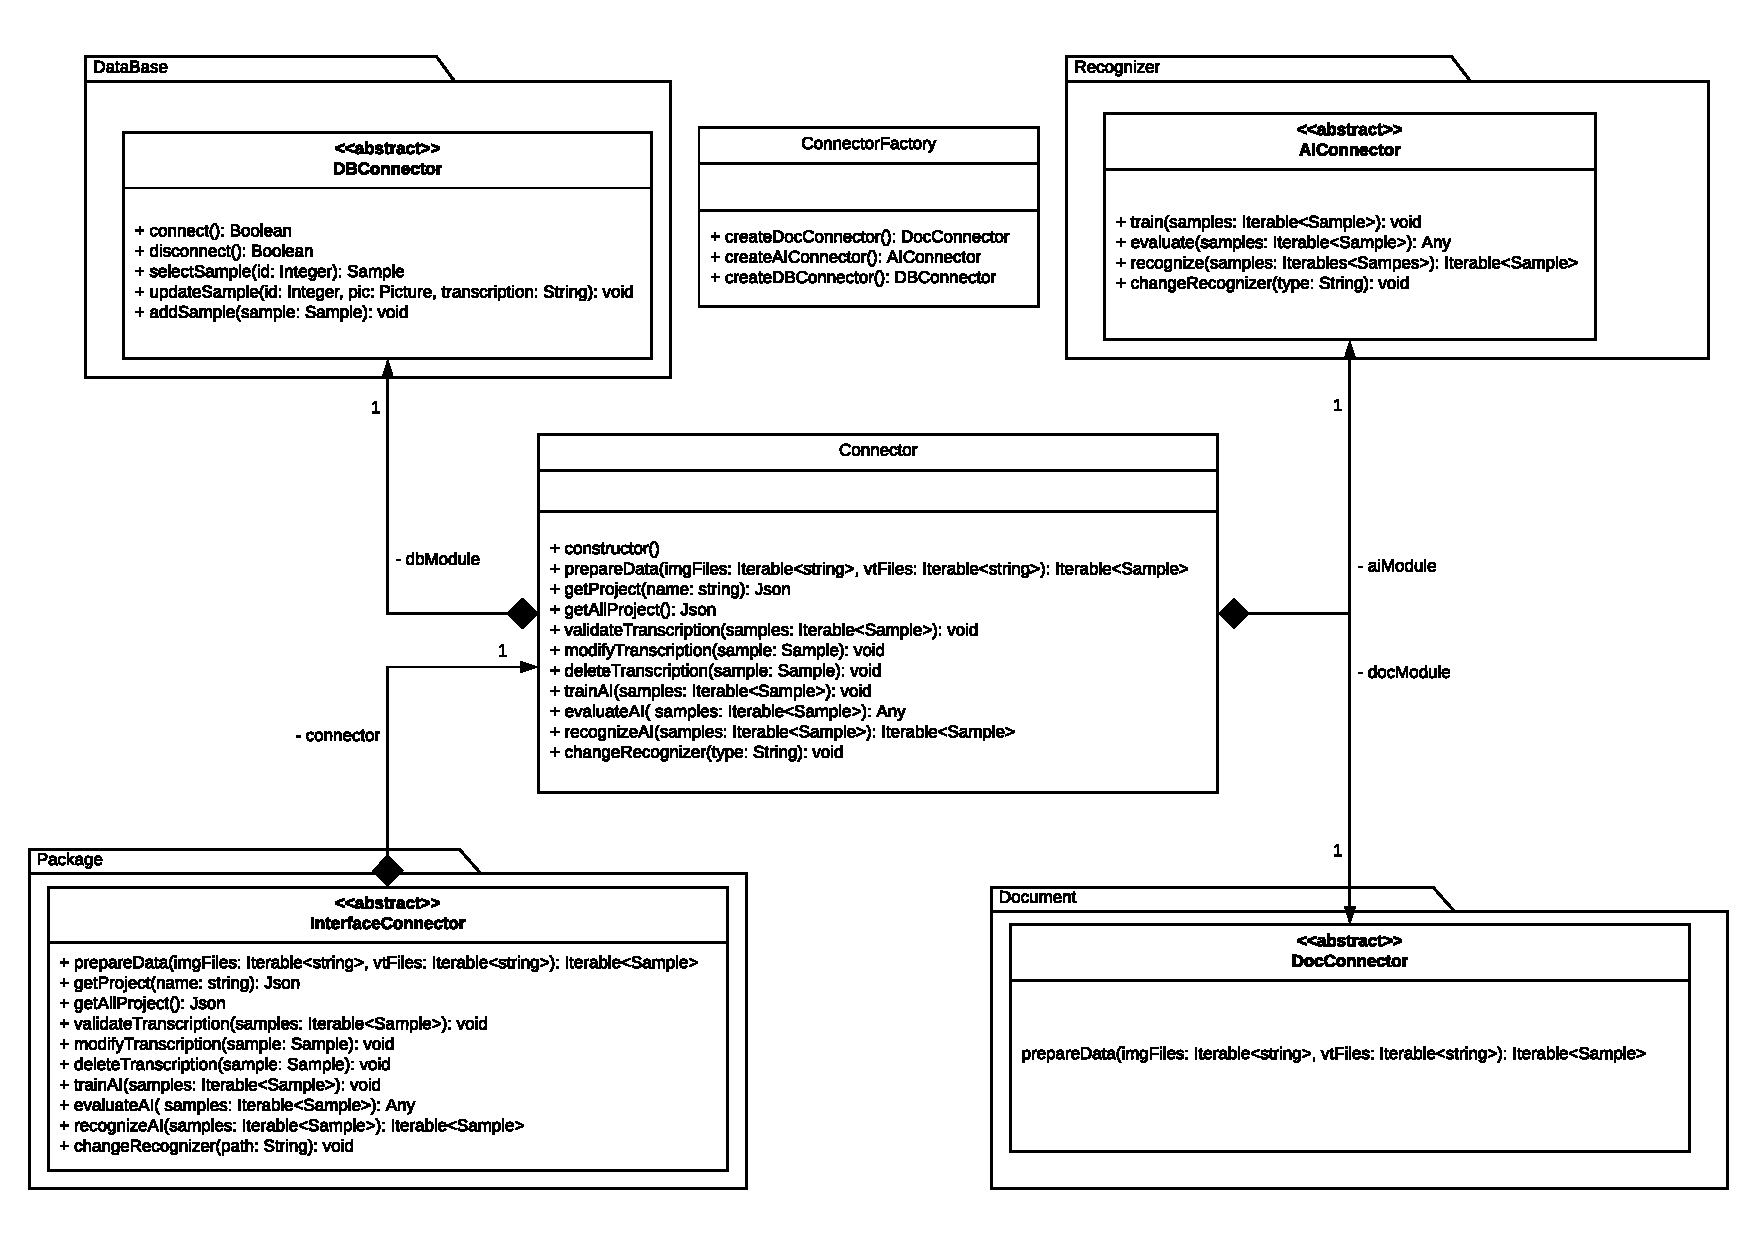
\includegraphics[trim={10cm, 0, 6cm, 0} ,scale=0.25]{assets/UML_connecteur.pdf}
\end{center}
\end{mdframed}

\paragraph{}
Dans notre projet, nous aurons également besoin de représenter les objets avec lesquels nous travaillons. Ainsi, nous avons choisi d'implémenter des classes de données pour représenter les exemples d'apprentissage (\texttt{Example}), les pages des documents utilisés (\texttt{Page}), lesdits documents (\texttt{Document}) et enfin les projets (\texttt{Project}) car on peut imaginer que l'utilisateur puisse vouloir avoir un projet sur des archives paroissiales et un autre sur des textes arabes anciens.

\begin{mdframed}[frametitle={Figure 9 : Structure du package de données}, innerbottommargin=10]
\begin{center}
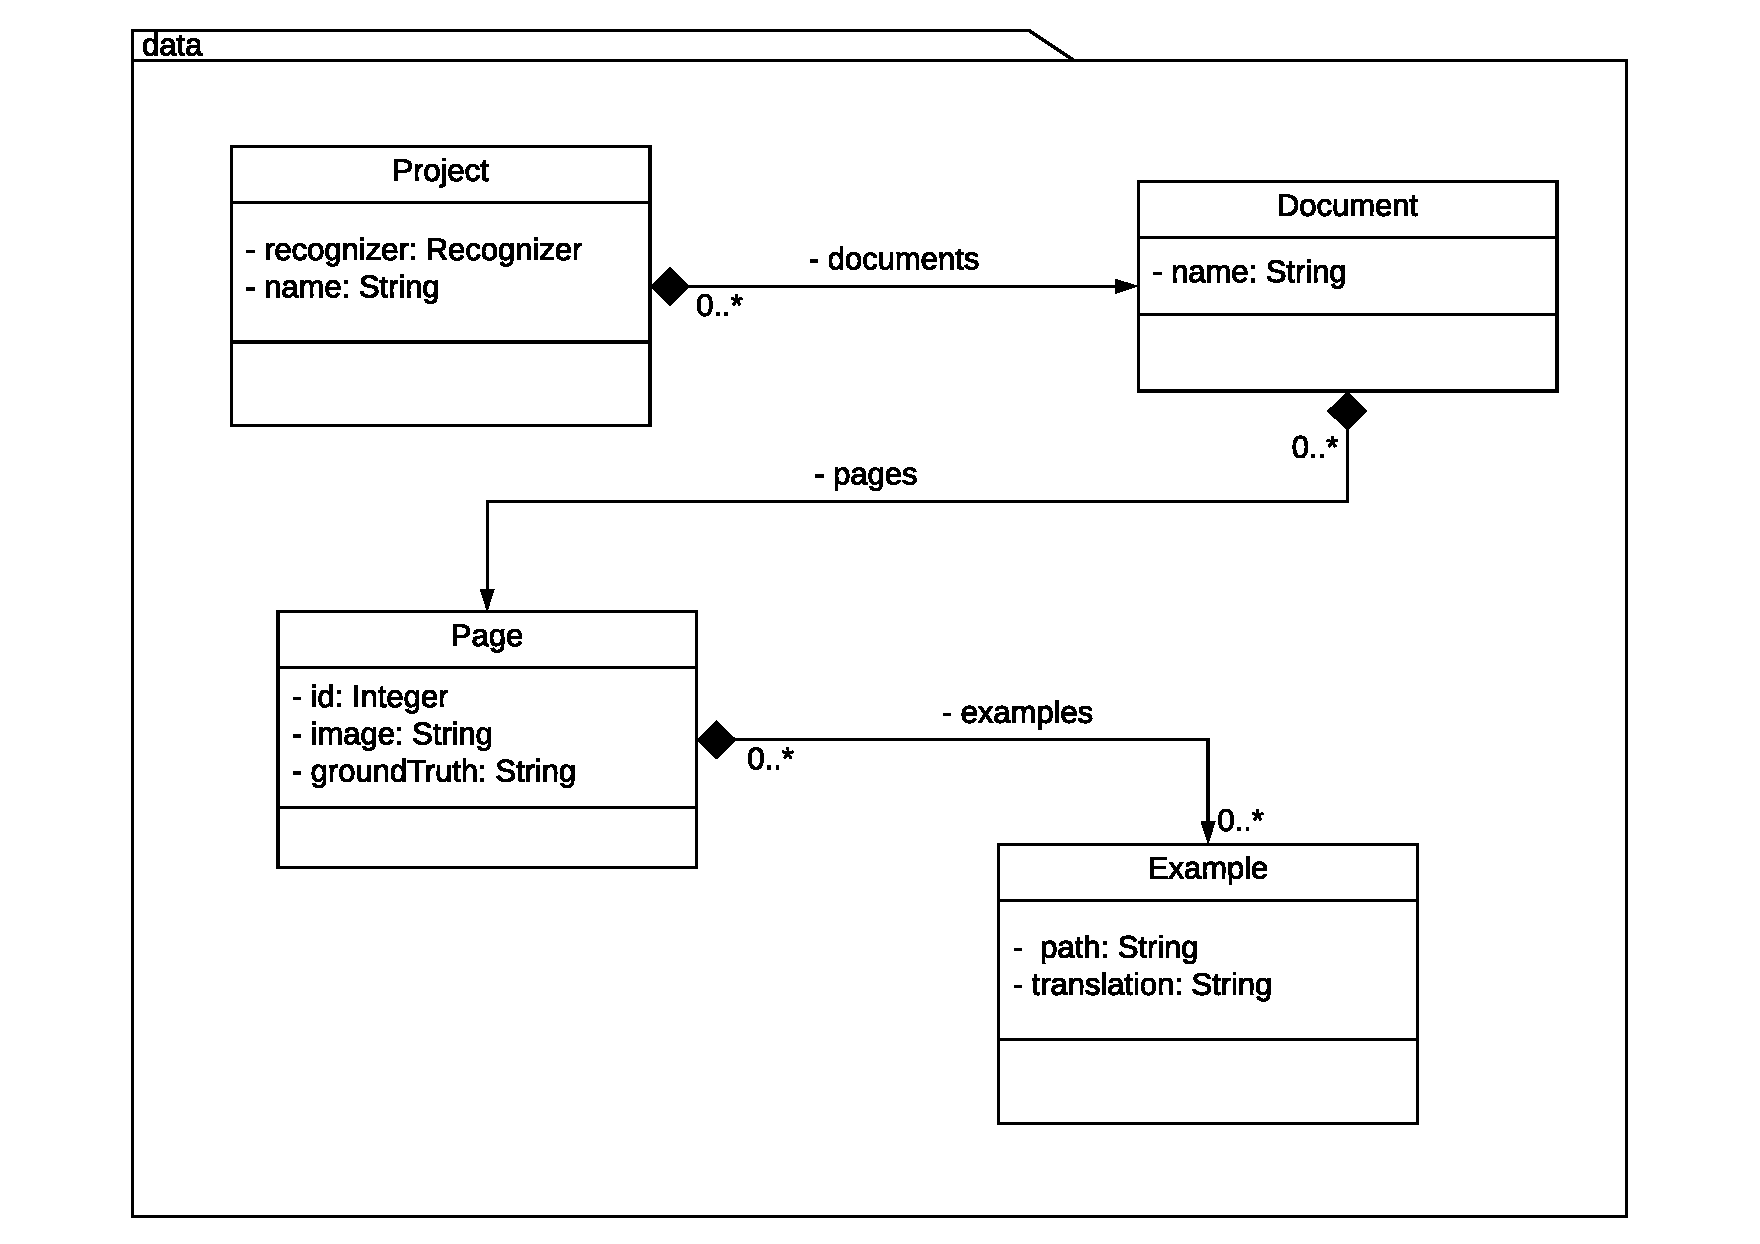
\includegraphics[scale=0.4]{assets/UML_data.pdf}
\end{center}
\end{mdframed}

L'attribut \texttt{Recogniser} est converti en \texttt{String} dans la base de données en passant par un \textit{enum} recensant les différents reconnaisseurs existants. Ces classes de données sont liées à la structure de la base de données et seront donc expliquées plus profondément dans cette partie.

\section{Technologies}



\subsection{Serveur}

Le serveur étant un ensemble de modules, chaque module utilise une technologie différente en lien avec sa fonction. Nous aborderons en premier les technologies nécessaires à la préparations des données, puis sur celles liées à leur stockage. Nous verrons ensuite celles utilisées par l'API Rest développée pour communiquer avec le client et enfin, celles de l'interface avec le reconnaisseur.

\subsubsection{Préparation des données}

Pour gérer la découpe des images, nous avons décidé d'utiliser la bibliothèque OpenCV car celle-ci fournit des outils de découpe et de traitement d'image adaptés à ce que nous souhaitions faire.

\subsubsection{Stockage des données}

Pour stocker les données, nous avions décidé de nous orienter vers un système de gestion de base de données. Nous avions décider, par simplicité et du fait que peu de contraintes (demandes d'accès simultanés, lourd nombre d'image) allaient s'imposer à ce système, de choisir un gestionnaire de base de données n'utilisant pas de serveur et local. Ce qui nous a fait porter notre choix sur Sqlite qui est une technologie simple d'utilisation avec une bibliothèque d'interfacage avec java facile à prendre en main.

\subsubsection{API Rest}

Ayant fait le choix d'utiliser un client Web, nous avons alors du réfléchir à developper une API Rest afin que le client puisse effectuer ses requêtes sur le serveur. Il nous fallait tout d'abord établir un serveur qui serait en mesure de recevoir des requêtes Http en provenance du client. Notre choix s'est alors porté sur Grizzly et Jersey que nous avons utilisé dans un projet précédent en java. Il nous fallait également de quoi construire et déconstruire nos objects locaux au serveur en json afin de pourvoir les transmettre au client. Nous avons alors choisi d'utiliser la bibliothèque org.json qui répond à ces problèmes.

\subsubsection{Interface avec le reconnaisseur}

Nous avons décidé de permettre à l'utilisateur d'utiliser un reconnaisseur afin de proposer une première transcription des imagettes afin de permettre plus d'ergonomie dans l'utilisation de l'application. Pour cela, il nous a été proposé d'utiliser Laia qui est un système de reconnaissance d'écriture manuscrite

\subsection{Client}

Concernant le client, nous avons opté pour une application Web afin de permettre une évolution vers un possible contexte multiutilisateur dans le cas où notre projet serait deployé sur un serveur distant et d'où les utilisateurs y accèderaient au travers d'une page web. De nombreux framework web existent et nous avons choisi d'utiliser Angular7, soit la dernière version de celui-ci. Nous avions déjà utilisé ce framework durant un projet précédent ce qui ne nous obligeait pas à réapprendre un nouvel outil, mais à consolider les bases que nous avions dessus afin d'avoir au plus vite une version fonctionnelle. De plus, il possède une bonne documentation et de nombreux guides existent.